\documentclass{article}

\usepackage{tikz}
\usetikzlibrary{arrows.meta,babel,calc,intersections,through,backgrounds,angles,quotes}

\title{Connecting path with arcs}

\begin{document}

\maketitle

We want to connect rail tracks with continuous curves, but Bezier curves and B-splines suffer from the problem that they cannot calculate the exact length.
It is problematic for us because we are using the distance to interpolate nodes in a constant interval, and also predict the distance to decelerate.
So we consider using arcs, which are sections of circles that have a constant curveture over its span.

\begin{figure}
\centering
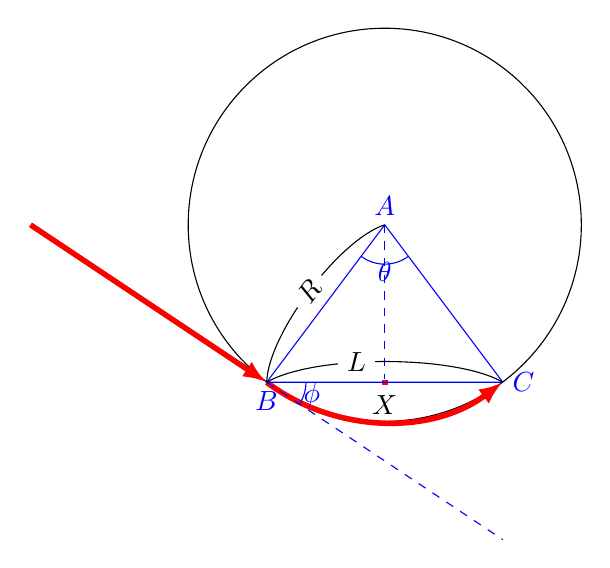
\begin{tikzpicture}
    \coordinate (O) at (-3/2-4/2*3/2,0);
    \coordinate [label=above:\textcolor{blue}{$A$}] (A) at (0,0);
    \coordinate [label=below:\textcolor{blue}{$B$}] (B) at (-3/2,-4/2);
    \coordinate [label=right:\textcolor{blue}{$C$}] (C) at (3/2,-4/2);
    \coordinate (D) at ($(B) + (B) - (O)$);
    \node [fill=red,inner sep=1pt,label=below:$X$] (X) at ($ (B)!.5!(C) $) {};
  
    \draw (A) let
      \p1 = ($ (B) - (A) $)
    in
      circle ({veclen(\x1,\y1)});

    \draw[line width=2pt, -{Latex[length=3mm]}, red] (O) -- (B);

    \draw[line width=2pt, -{Latex[length=3mm]}, red] (B) let
        \p1 = ($ (B) - (A) $),
        \p2 = ($ (C) - (A) $),
        \n1 = {veclen(\x1,\y1)},
        \n2 = {atan2(\y1,\x1)},
        \n3 = {atan2(\y2,\x2)}
    in
        arc [start angle=\n2, end angle=\n3, radius=\n1];

    \draw[blue] (C) -- (B) -- (A) pic[draw=blue, angle eccentricity=1.2, angle radius=0.5cm, "$\phi$"] {angle=D--B--C};
    \draw[blue] (A) -- (C) pic[draw=blue, angle eccentricity=1.2, angle radius=0.5cm, "$\theta$"] {angle=B--A--C};
    \draw[blue,dashed] (A) -- (X);
    \draw[blue,dashed] (B) -- (D);

    \draw (A).. controls ($(A)!.2!(B)!10pt!-90:(B)$) and ($(A)!.8!(B)!10pt!-90:(B)$) .. (B) node [midway, sloped, fill=white] {$R$};
    \draw (B).. controls ($(B)!.2!(C)!10pt!90:(C)$) and ($(B)!.8!(C)!10pt!90:(C)$) .. (C) node [pos=0.4, fill=white] {$L$};
\end{tikzpicture}
\caption{The arc section and smooth connection from incoming path. The red arrows indicate the path from previous section and the arc.}
\label{fig:arc}
\end{figure}

In figure \ref{fig:arc}, we denote the center of the circle of the arc as $A$.
The point at which the previous path ends is denoted as $B$.
We would like to continue the path from $B$, keeping the direction continuous (i.e. $C^1$ continuous).

Let's say the user clicked on the point $C$.
We would like to find the parameters of the arc, which are:
\begin{itemize}
    \item $A$ - center of the arc circle
    \item $R$ - the radius of the curve
    \item $\theta$ - the angle of the arc.
\end{itemize}

Let's call the direction change from the point $B$ to $C$ as $\phi$.
We can compute $\phi$ from the clicked point $C$ like
$$
\phi = \arctan\left({\frac{C_y - B_y}{C_x - B_x}}\right) - \phi_0
$$
where $\phi_0$ is the angle of direction from previous path.

We can also compute the distance between $B$ and $C$ as $L = ||\vec{BC}||$.

From $\phi$ and $L$, we can calculate the radius as
$$
R = \frac{L}{2 \sin\phi}.
$$

With some simple geometry, we observe that $\theta=\frac{\phi}{2}$.

With all these information, you can determine the arc.

\end{document}
